% 47-16(47쪽) — $y=\log_2 x$ 의 그래프와 직선 $y=x$, $x$축 위의 $1$·$a$·$b$·$c$·$d$ 와 점선(원문 「오른쪽 그림」).
% 스캔 화질이 낮아 TikZ 로 다시 그림. 점선은 원문대로 $a\to b$, $c\to d$ 두 벌 — 직선 $y=x$ 위의 점에서 가로로 가 곡선에 닿고 거기서 세로로 $x$축에 내려온다.
% 라벨은 원문에 있는 것만 — $y=x$ · $y=\log_2 x$ · $\pt{O}$ · $1$ · $a$ · $b$ · $c$ · $d$ · $x$ · $y$. 값(답)은 적지 않는다.
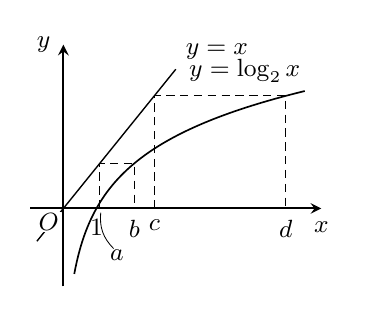
\begin{tikzpicture}[line width=0.6pt, x=0.42cm, y=0.52cm, >=stealth]
  \draw[->, line width=0.7pt] (-1.0,0) -- (7.8,0) node[below=1pt, font=\small] {$x$};
  \draw[->, line width=0.7pt] (0,-1.9) -- (0,4.0) node[left=1pt, font=\small] {$y$};
  \draw[line width=0.5pt] (-0.8,-0.8) -- (3.4,3.4);
  \draw[domain=0.33:7.3, samples=160, smooth] plot (\x, {ln(\x)/0.693147});
  \draw[densely dashed, line width=0.3pt] (1.1,0) -- (1.1,1.1) -- (2.1435,1.1) -- (2.1435,0);
  \draw[densely dashed, line width=0.3pt] (2.75,0) -- (2.75,2.75) -- (6.7272,2.75) -- (6.7272,0);
  \node[font=\small, fill=white, inner sep=0.6pt, anchor=north east] at (-0.06,-0.06) {$\pt{O}$};
  \node[below=0pt, font=\small] at (1,-0.03) {$1$};
  \node[below=0pt, font=\small] at (2.1435,-0.03) {$b$};
  \node[below=0pt, font=\small] at (2.75,-0.03) {$c$};
  \node[below=0pt, font=\small] at (6.7272,-0.03) {$d$};
  \node[font=\small] at (1.62,-1.15) {$a$};
  \draw[line width=0.3pt] (1.52,-0.98) to[bend left=25] (1.13,-0.10);
  \node[anchor=south west, font=\small] at (3.40,3.40) {$y=x$};
  \node[anchor=south west, font=\small] at (3.50,2.83) {$y=\log_2 x$};
\end{tikzpicture}
